% !TeX program = xelatex
% 编译：在 report 目录执行 latexmk -xelatex report.tex
\documentclass[UTF8,a4paper,11pt,fontset=fandol]{ctexart}
\usepackage[margin=2.2cm]{geometry}
\usepackage{graphicx}
\graphicspath{{imgs/}{report/imgs/}}
\usepackage{booktabs}
\usepackage{array}
\usepackage{caption}
\usepackage{listings}
\usepackage{xcolor}
\usepackage[hidelinks]{hyperref}

\setlength{\parindent}{0pt}
\setlength{\parskip}{0.4em}
\renewcommand{\arraystretch}{1.1}
\captionsetup{font=small}
\ctexset{
  section={format=\Large\bfseries,beforeskip=1em,afterskip=0.5em},
  subsection={format=\large\bfseries,beforeskip=0.8em,afterskip=0.4em}
}
\lstset{
  language=C,
  basicstyle=\small\ttfamily,
  keywordstyle=\color{blue!50!black},
  commentstyle=\color{black!55},
  backgroundcolor=\color{black!3},
  frame=single,
  rulecolor=\color{black!20},
  framesep=5pt,
  columns=fullflexible,
  keepspaces=true,
  showstringspaces=false,
  breaklines=true,
  aboveskip=0.5em,
  belowskip=0.5em
}

\begin{document}

\begin{center}
  {\LARGE\bfseries DataLab 实验报告}
\end{center}

姓名：唐培元\hfill
学号：2025201805

\textbf{测试成绩：37/37，全部 12 个函数通过测试。}

\begin{center}
\small
\begin{tabular}{>{\ttfamily}lccc}
\toprule
\multicolumn{1}{l}{函数} & 得分 & 满分 & 测试结果 \\
\midrule
bitAnd       & 1  & 1  & PASS \\
bitXor       & 1  & 1  & PASS \\
samesign     & 2  & 2  & PASS \\
logtwo       & 4  & 4  & PASS \\
byteSwap     & 4  & 4  & PASS \\
reverse      & 3  & 3  & PASS \\
logicalShift & 3  & 3  & PASS \\
leftBitCount & 4  & 4  & PASS \\
float\_i2f   & 4  & 4  & PASS \\
floatScale2  & 4  & 4  & PASS \\
float64\_f2i & 3  & 3  & PASS \\
floatPower2  & 4  & 4  & PASS \\
\midrule
\multicolumn{1}{l}{\bfseries 总分} & \textbf{37} & \textbf{37} & \textbf{PASS} \\
\bottomrule
\end{tabular}
\end{center}

\textbf{test 截图}

\begin{figure}[htbp]
  \centering
  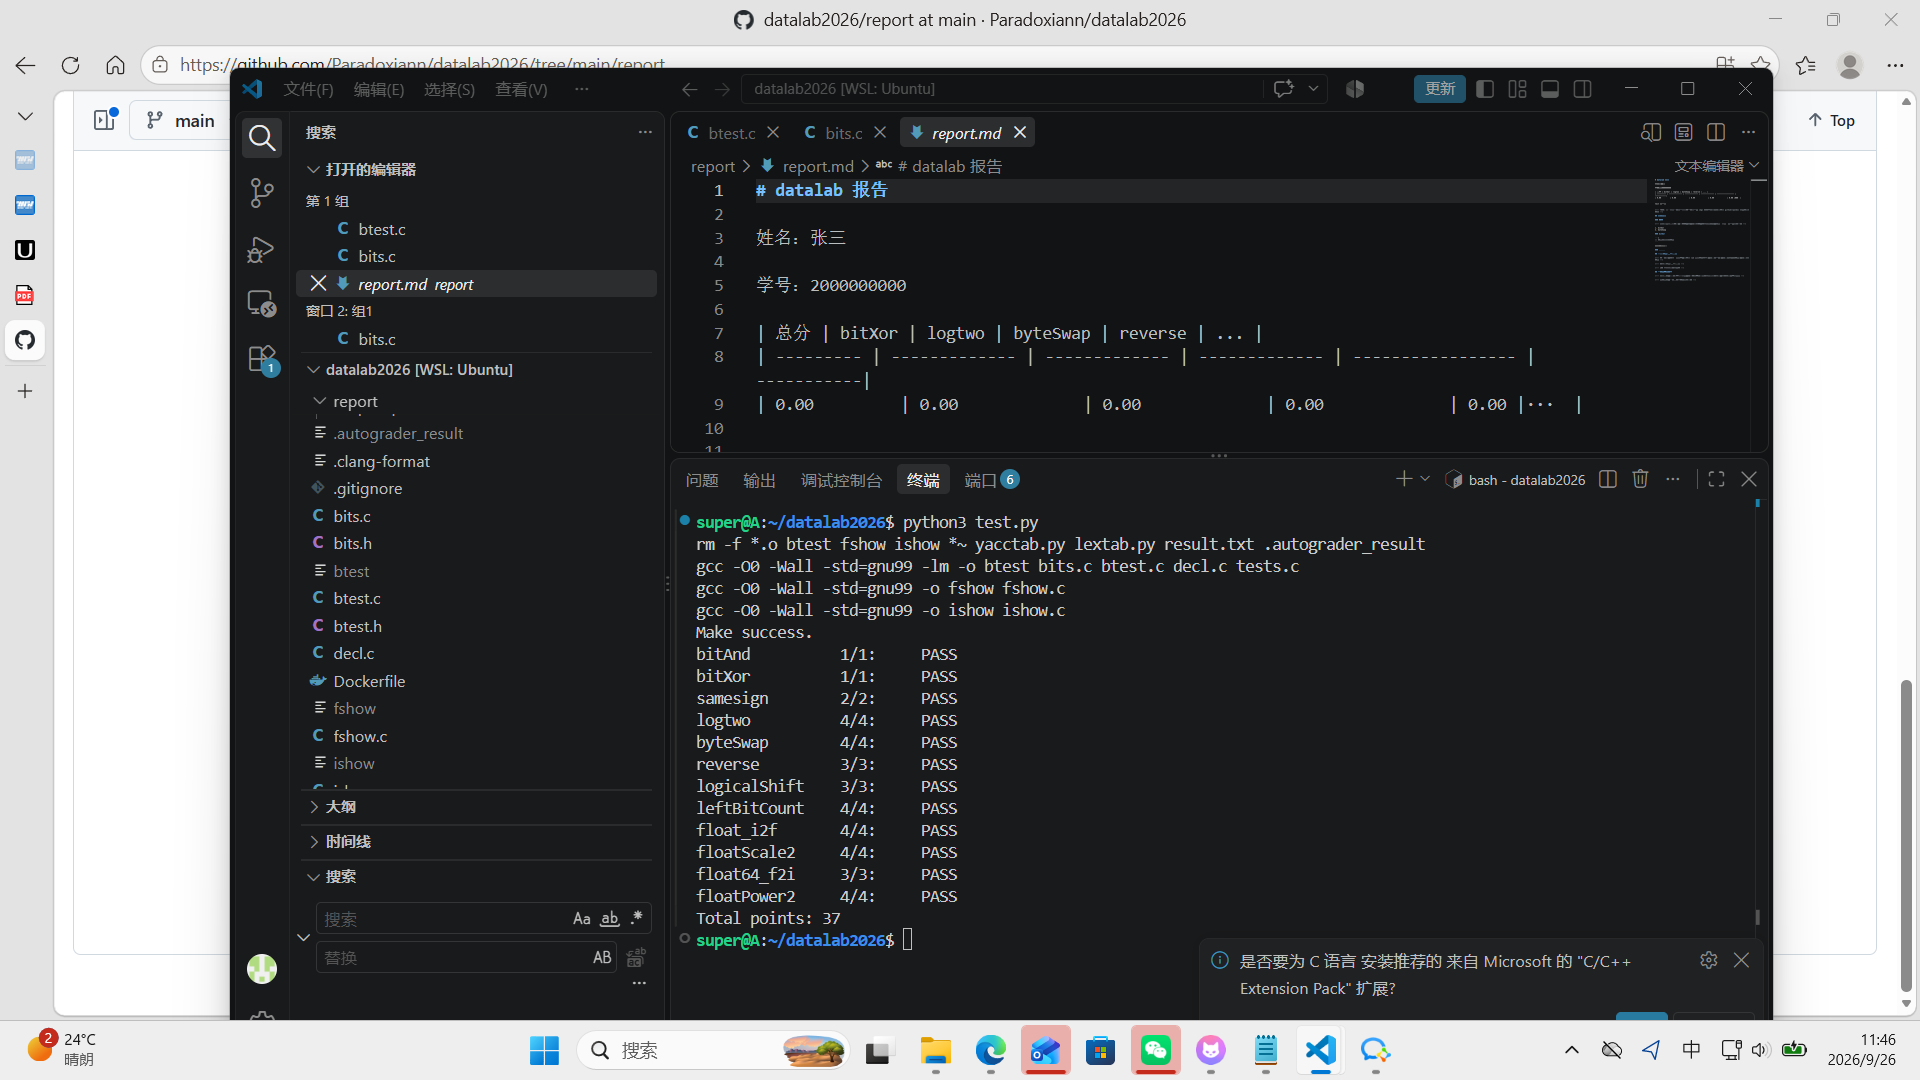
\includegraphics[width=0.78\textwidth,
    trim=408bp 73.8bp 330bp 294bp,clip]{test.png}
  \caption{DataLab 测试结果}
\end{figure}

\clearpage
\section{解题报告}

\subsection{亮点}

\begin{enumerate}
  \setlength{\itemsep}{0pt}
  \setlength{\parskip}{0pt}
  \item \texttt{float\_i2f}
  \item \texttt{float64\_f2i}
  \item \texttt{floatScale2}
  \item \texttt{leftBitCount}
  \item \texttt{logicalShift}
\end{enumerate}

\subsection{\texttt{float\_i2f}}

首先特判 \texttt{x == 0}，防止后面的循环无法终止。
用 \texttt{sign} 和 \texttt{absx} 分别记录符号和绝对值，
再结合 \texttt{for} 循环，用 \texttt{mark} 记录最高有效位距离第 31 位的位置，
通过 \texttt{pow = 31 - mark} 得到实际指数。

\begin{lstlisting}
unsigned norm = absx << mark;
unsigned keep = norm >> 8;
unsigned lost = norm & 0xFF;
\end{lstlisting}

这里直接将最高有效位移到第 31 位，在固定位置截取保留部分和舍弃部分。
相比代码中已注释的初版实现，这种写法避免了复杂的动态截断和移位，
减少了操作数，也提高了可读性。

接着将 \texttt{lost} 与 \texttt{0x80}（舍弃部分的一半）比较，完成舍入判断：
大于一半时进位；恰好等于一半时，根据 \texttt{keep} 的最低位决定是否进位，
实现取偶数舍入。满足条件时执行 \texttt{keep = keep + 1}。
这比初版分别判断第一位舍弃位和其余舍弃位是否为零更简洁。

最终返回：

\begin{lstlisting}
return sign + ((pow + 126) << 23) + keep;
\end{lstlisting}

这里使用 \texttt{pow + 126} 而不是 \texttt{pow + 127}，
是因为 \texttt{keep} 保留了有效数 $1.xxx$ 前面的 $1$。
该位位于第 23 位，通过加法自然为指数补上 $1$。
此外，当保留部分全为 $1$ 且舍入仍需进位时，
进位也会自然进入指数区域，无需额外特判，节省了操作数。

\subsection{\texttt{float64\_f2i}}

直接使用手算得到的掩码，例如 \texttt{0x80000000}、
\texttt{0x000FFFFF} 和 \texttt{0x7FF00000}，减少了构造掩码消耗的操作数。

对于 \texttt{pow >= 31} 的情况，无论是 $-2^{31}$ 还是溢出，
返回值的位模式都为 \texttt{0x80000000}，因此可以统一处理，减少额外判断。
最终共使用 17 个操作，少于题目允许的 60 个。

\subsection{\texttt{floatScale2}}

对于指数为零的情况，统一将尾数部分 \texttt{M} 左移一位。
对于零，移位后保持不变；对于非规格化数，
若尾数移位产生进位，该位会自然进入指数区域，使指数变为 $1$。
利用这样的位布局关系，不需要额外判断是否转为规格化数。

\subsection{\texttt{leftBitCount}}

\begin{lstlisting}
x = ~x;
\end{lstlisting}

先将 \texttt{x} 取反，把求左侧连续 $1$ 的问题转化为求左侧连续 $0$。
这样，对于一段待检查的位，只需判断其整体是否为零，
即可判断它们是否全部为 $0$；而对于连续 $1$，不能直接通过零值判断做到这一点。

\subsection{\texttt{logicalShift}}

\begin{lstlisting}
int temp = x >> n;
// int mask = (1 << (32 + (~n + 1))) - 1;
int mask = ~((1 << 31) >> n << 1);
return temp & mask;
\end{lstlisting}

若使用注释中的常规构造方法，当 \texttt{n = 0} 时，
会出现左移 32 位的问题。
当前方法利用实验中负数补码的算术右移构造掩码，避免了移位量为 32 的情况。

\section{反馈／收获／感悟／总结}

花费的时间远长于预期。我认为这种思维很反直觉，写起来极度不舒适，
经常像在做以最小化操作数为目标的优化问题，
使我更倾向于写嵌套的 \texttt{if}，而非通过 \texttt{\&\&} 连接条件。

我感受到了构造掩码的重要作用，筛选特定位通常都需要它；
也体会到了位关系的重要性，可以利用位布局实现相邻、含义不同的字段之间的自然进位。

\section{参考的重要资料}

课程课件 \texttt{3\_encoding.pptx}，第 97 页：
使用布尔值和位运算实现与相应 \texttt{if} 等效的功能，以及二分查找的使用。

\end{document}
